\chapter{System Design / Work Done}\label{C:work_done}

\section{Characteristics}

The main factor of this project is that it focuses on a mobile application, rather than a website application. This forces some limitations in terms of how users will interact with the system, since with a mobile interface, the small form factor affects many changes which will be described later on. Since existing components of WOTM are done in the programming language Ruby, it means we are confined to this language. In addition, the data in the application has already been modelled, including the dishes, restaurants, users and so on. The only data that had not been modelled was the data required for the recommender system such as like/dislikes and preferences.   

\section{Design Decisions}

\subsection{Open source projects}
This section identifies the open source projects that were considered for this project.

Open source projects can be utilised to fit the projects specific needs, as opposed to the alternative of starting from scratch. This saves time, allowing the focus to be on the CF techniques themselves. The open source community has a range of available projects. In particular, a range of machine learning libraries are available that incorporate various types of CF techniques. Spotify \cite{annoy} have an open-source project called Annoy \cite{annoy} that uses a CF neighbourhood approach. Recommendable \cite{recommendable} also uses a CF neighbourhood approach and is written in Ruby, making it easy to setup with the existing WOTM components \cite{recommendable}. There were many other open-source projects such as EasyRec \cite{easyrec}, Apache Mahout \cite{mahoutaction}, Lenskit \cite{lenskit}, and so forth, containing a range of CF techniques. 

Investigations on these systems led to the discovery of PredictionIO, the main open-source project used in this project. The following section explains the reasons why PredictionIO was chosen. 

\subsubsection{PredictionIO}

PredictionIO is an open-source machine learning server used to ``build and deploy predictive applications in a fraction of the time" \cite{predictionio, predictionio2}.

\begin{figure}
\centering
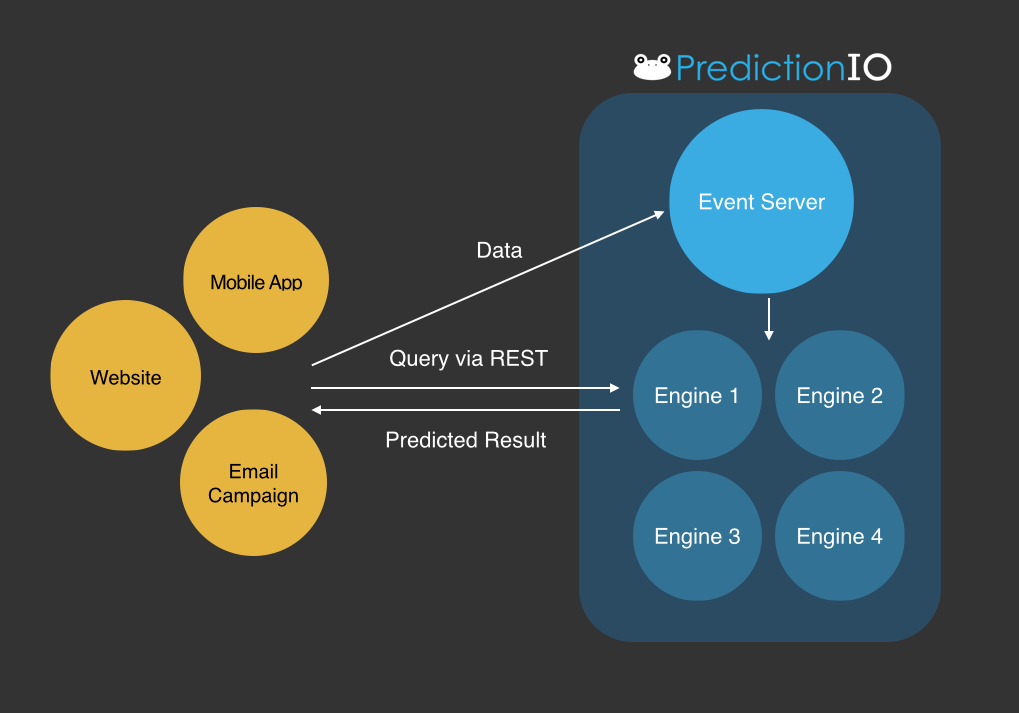
\includegraphics[scale=0.35]{images/predictionIO}
\caption{ How external applications interact with PredictionIO \cite{predictionio}. In this case, WOTM can interact with PredictionIO through REST queries which enable communication and data between the two applications.}
\label{fig:predictionIO}
\end{figure}


Figure \ref{fig:predictionIO} represents how PredictionIO is made to integrate with existing applications \cite{predictionio}. Data such as rating events from WOTM is sent to the Event Server where it is stored on PredictionIO. PredictionIO uses a distributed database that is easily scalable. Data from the event server is then used by algorithms from the engines to learn recommendations. These engines are deployed as distributed web services. WOTM can query these deployed engines to retrieve the top N recommendations for a specific user. 

The main advantage of using PredictionIO is that engines can be easily swapped out making it easy to examine and evaluate various CF techniques. This saves time, switching the main focus on CF algorithms rather than configuring settings to accommodate various technology and tools.

Additionally, these engines implement a DASE architecture. DASE stands for Data, Algorithms, Serving, and Evaluator. These components are considered to be independent in the engine which allows for separation of concerns. Implementation of various algorithms can be applied at the Algorithms stage, and enables results from the various algorithms to be combined at the Serving stage to produce hybrid CF approaches for recommendations.

PredictionIO already contains a range of customizable engines, including engines that use ALS techniques for CF. The PredictionIO community is active and new engines are frequently being produced. There is concise documentation in addition to support available. For these reasons, we found PredictionIO to be our best candidate and decided to use it. 

% \subsection{Online Learning vs Offline Learning}

% In a mobile application, speed and performance of recommendations is arguably more important than the prediction-accuracy. For instance, a user is more likely to use an application that provides fast recommendations to the users but less accurate recommendations, as opposed to an application that provides slow recommendations to the users but are accurate. In this case, the former is to be more accepted because users are able to easily skip inaccurate recommendations, whereas in the latter, users will have to wait for the recommendations to appear which may cause their attention to drift. 

% With this in consideration, it is important to provide fast recommendations to users, thus a model-based approaches would be more appropriate than neighbourhood methods. A model-based CF approach means that a model can be constructed and trained offline. Once the model is deployed, it will provide instant recommendations to the users because less computation needs to be done in real time, since the model has learnt what the user likes offline. As well as this, a model based approach means that expensive computation can be computed offline, providing high scalability. However, the disadvantage of a CF model based approach is that it must be regularly trained to take into account the recent new actions of the users. Therefore, regular intervals to train the model need to be defined depending on how often users rate dishes.

% Neighbourhood methods of CF perform online learning, meaning that they do the computation in real time. For instance, in user-based CF when a user likes a dish, then the algorithm will be performed then and there, finding similar users, then finding neighbours that are similar to that user, providing a recommendation. This technique is easy to implement, but does not scale well, and is slower than the modelled approach. However, depending on the size of data that is expected to be collected from this 'WOTM', it may be a valid approach if the data is not expected to be large (millions of ratings). As new users and new items grow in the application, it is expected that the amount of ratings will exponentially grow as well, therefore there is a possibility that scalability may have to be considered in the long term. As of now, we will focus on the performance of the recommender system.  

% For this reason, we will examine both online learning and offline learning, and see how implementations of the CF algorithm affect the performance of the recommendations that are produced.  


\subsection{User Experience}

A mobile application encourages user interaction that differs from that of a website. For instance, users are encouraged to use touch events to navigate through pages or to perform certain actions. This leads to design decisions that accommodate such interactions, making it easier for users to perform tasks on mobile applications. The user experience of WOTM affects how rating data is collected from users, which can affect the recommendation system. The following section explains the design decisions for collecting data events from users, and how these events can affect the recommender system. 

\subsection{Explicit Feedback}

Recommender systems rely on different types of input data \cite{koren2009matrix}. Explicit data is referred to as a direct record of someones interest of an item. For example, Netflix collects star ratings for movies, and TiVo users collect data from having a thumbs up or thumbs down directly indicating that they like or dislike a particular item \cite{koren2009matrix}. These events are mapped directly in the ratings matrix, and explain directly how a user feels about an item. 
The next section explains the design decisions regarding the explicit feedback we will collect in the WOTM application.

\subsubsection{Boolean Ratings vs Ternary Ratings vs Likert Scale Ratings}

Although prediction-accuracy is important, it is not the only factor that a recommender should focus on, and acts as one facet in wide range of facets \cite{martin2009recsys}. \citeauthor{martin2009recsys} explains that the goal of a recommender system is to improve user experience, however, designing a recommender system to fit a specific application remains a challenge, and recommender system ratings should be based on the user experience \cite{martin2009recsys}. By focusing on user experience, users will be able to easily rate food dishes, in turn, leading to the system collecting more information for the recommender system from ease of use. For this reason, a simple model allowing users to easily rate a dish such as a binary rating (Like/Neutral) or a ternary rating (like/neutral/dislike) is preferred over Likert scale ratings. This provides simplicity, but means recommendations will not be as accurate as Likert scale ratings such as 1-5 stars or 1-10 stars. By easing the user experience for rating food dishes it can increase data collection at the expense of accuracy. In fact, \citeauthor{movieratings} found that users provided more ratings that had options to ``like" or ``dislike" than users with only one rating option \cite{schafer2007collaborative, movieratings}. 

Using Likert scaled ratings mean that we learn more about the user preferences because of the scaled factor indicating how much the user likes a dish or not. This means that model based CF techniques are able to learn what the user likes and dislikes faster leading to more accurate recommendations. However, a Likert scale system such as a 1-5 star rating also has problems. For example, if a dish had a 5 star rating, it may mean only 1 or 2 people have rated the dish. Ratings such as 3.5 stars may mean that it is a good dish, but from the way it is displayed, may seem otherwise. \citeauthor{interface} explains that by displaying what other users think of an item, the active user tends be influenced by the opinions of others, leading to bias ratings \cite{interface}. An example would be a user rating a dish higher than they would normally because the food dish has an average of 4.5 stars. This can lead to inaccurate recommendations for the active user in the long term, because users may be influenced by others opinion \cite{interface}. \citeauthor{interface} argues that the way ratings are collected, and displayed influence how others will rate the dish. Considerations like this have to be taken into account to understand how the user will perceive and interact with the recommender system.  

A trade-off to consider is whether or not accurate recommendations are more important than the user experience. Since WOTM aims at being a mobile application, the limitations are the small form factor that mobile phone screens have. With a Likert scale rating system, the user has to be shown these possible options in order to rate a dish. This can take up additional space that is not available on small screens. Because of this, having a 1-5 star rating system may degrade the user experience as opposed to a simple like/dislike rating system. 

For a mobile application, the predicted score of the recommender system may not matter a great deal. For instance, a recommender system could predict two dishes the user may like based on previous rating patterns. The first dish is predicted with a 90\% predicted score, and the second dish is predicted with a 70\% predicted score that the user will like these dishes. But is the difference in prediction scores important if the user likes both dishes? As long as the recommender system has provided the user with dishes they like, the accuracy between those predicted dishes do not drastically matter. In addition, dishes with higher predicted scores may seem like obvious choices the user may have already tried, whereas dishes with a lower predicted score may lead to less obvious dishes that they may like, but have not tried yet. A recommender system using boolean or ternary values may eventually reach prediction accuracy similar to using likert scale ratings. Although this will happen in the long term, new ratings will most likely lead to less accurate predictions that join the system in the short term until more ratings are collected. 

Foursquare is an application that asks users to rate items according to a series of questions. These questions consist of ``What do you like about this place?", ``What is this place known for?" and so on. From these questions they are able infer a particular rating for the item, as well as collect data from users to give more accurate recommendations. This rating system may risk users not rating the items because of the long list of questions it asks. \cite{martin2009recsys} explains that part of the challenge is to design interfaces ``that give users control over the recommendation process without overwhelming the user or rendering the tool too complicated for novice users." 

For these reasons, we found that simple like/dislike events would best suit the collection of data for the recommender system because of the simplified structure which increases the user experience. The recommender system can be extended to take in additional events that may portray additional information such as a ``want" indicating that a user ``wants" a dish but has not yet tried it before. However, caution must be taken as more events will affect the user experience of the application, but may lead to more accurate recommendations. 

\subsection{Implicit Feedback}

When explicit feedback is not available, implicit data can be used to infer preferences from users \cite{koren2009matrix}. Implicit feedback is referred to as an indirect reflection of someones interest in an item. Implicit feedback can be from observing user behaviour. This could include click through data, browsing history, the way users react to certain events, search patterns, and so on \cite{koren2009matrix}. Implicit feedback can be collected to increase the accuracy of recommendations to users by being combined with explicit feedback, or can fill in the ratings matrix when explicit events are not available, alleviating the 'Cold Start' problem as it makes the matrix more dense. The next section explains design decisions regarding the implicit feedback in WOTM.

\subsubsection{Additional Events}

Netflix \cite{koren2009matrix} and other sites such as Amazon.com \cite{schafer2007collaborative} use implicit feedback such as views and purchase history in their recommender systems. These events indicate some form of interest in the user, however are less practical to apply for a mobile application. For example, on a website, many products are able to be shown to the user. When a user selects a product it will indicate some form of implicit feedback such as the user is interested in that product. With the WOTM mobile application, it can be diffiuclt showing a range of food dishes to users because of the small screen size. This can make it difficult to collect additional implicit feedback. As well as this, purchase history and similar events are not practical because users are unlikely to indicate that they have purchased a dish after they have tried it. Explicit events such as like and dislike already infer that they have tried the dish, which make purchase history redundant. The implicit event of commenting on a dish may provide valuable information, perhaps commenting on a dish means that there is a strong interest or disinterest a user has about a specific dish. However, this is impractical because we do not know if the comment is good or bad without using extraction techniques.

A consideration is how to collect feedback on how the user feels about the recommendations produced by the recommender system. This can be used to gather more events, to make predictions more accurate. For instance, a user can indicate that they liked/disliked the recommendation that was shown to them, or they could skip it altogether meaning that they do not have an opinion about it. Although the flaw in this method is that recommendations may be dishes the user has not tried yet. Therefore, they may keep skipping through recommendations and provide no valid feedback to them. Although this may happen, an assumption is that user ``Like" events may be used for a dish that the user has not yet tried, but is interested in. 

For these reasons, we do not use any implicit events in our recommendation system.

\section{Implementation}

This section explains what has been implemented according to the design decisions in the previous section.


\subsection{Latent Factor Models}

PredictionIO \cite{predictionio} provides many template engines, some of which use CF algorithms to make recommendations to users. In particular, there is a template engine that uses Alternating Least Squares, learning user preferences based on previous rating patterns. This engine is called the ``E-Commerce Recommendation Engine", and will be built upon to suit our user case. The following section explains the E-Commerce Recommendation Engine and the changes that have been made to it for this project. 

\subsubsection{E-Commerce Recommendation Engine}

The E-Commerce Recommendation Engine is written in the programming language Scala and is made to provide personalised recommendations for e-commerce applications. This engine uses Alternating Least Squares which is a model-based CF technique. This means that the model trains on the users rating patterns to learn about recommendations that the users may be interested in. Training occurs offline. The engine also comes with the following out of the box functionality \cite{predictionio}.
\begin{enumerate}
 \item Exclude out-of-stock items
 \item Provide recommendation to new users who sign up after the model is trained
 \item Recommend unseen items only (configurable)
 \item Recommend popular items if no information about the user is available
\end{enumerate}

\todo{Redo this}
Default events in the engine are view events and purchase events.
Since ``view" and ``purchase" ratings are implicit events and not explicit events such as Likert scaled ratings from values 1-5, the implicit events have to be represented differently in the ratings matrix. An implicit event such as ``view" or ``purchase" event maps to a binary preference value of 1. Missing events map to a binary preference value of 0. 

A binary preference value of 1 indicates that the user likes the item, and a binary preference of 0 indicates no preference for the user. Additionally, implicit events also have a confidence value associated with it. These confidence values represent the confidence levels of the binary preference values being true. In this case, preference values for the ``view" and ``purchase" events correlate to the value of 1. Multiple identical events such as a user viewing the same item multiple times correlate to higher confidence levels since the confidence level is an aggregation of preference values. This means that there is a higher confidence level that the binary preference value is true, in this case, that the user will like the item because the user viewed or purchased the same item multiple times, recommendations taking this into account \todo{how? how can this be calculated?}. 

\todo{Move this to the Hybrid Section}

Alternating Least Squares is then used with the same steps in equation \ref{eq:2}, except with a different minimization equation that considers the implicit events. This minimization equation is for implicit events which is the following \cite{implicit}.

\begin{equation}\label{eq:3}\tag{3}
\displaystyle min_{q*,p*} \sum_{ (u,i) \in K} c_{ui}(b_{ui} - q_{i}^T p_{u})^2 + \lambda (\| q_{i} \|^2 + \| p_{u} \|^2 )
\end{equation}

In this equation, \begin{math} c_{ui} \end{math} is the confidence level and \begin{math} b_{ui} \end{math} is the binary preference value. 

\subsubsection{Modifications to the Engine}

Using this template, we modified this engine to take into account ``Like" and ``Dislike" events, removing the view and purchase events. We modified the CF algorithm in the engine to consider a ``Like" event as positive result, giving it the preference value of a 1. In contrast, we made the algorithm in the engine consider a ``Dislike" event to be a negative result, giving it the preference value of a -1. Since users may be able change their minds about liking or disliking a dish, we modified the CF algorithm to only take into account the most recent like/dislike event that occurs from the user, if there are multiple identical like/dislike events on a dish from that user. Filtering in this recommendation system was also added. Users are now able to filter recommendations based on their preferences such as their meat type, their cuisine type, and their food type. As well as this, users can see recommendations that are within their price range, if specified. 

If dishes are no longer available, then we are able to send a query to the recommendation engine to tell it that the dish is unavailable. Another feature is that we are also able to send a query to the recommendation engine to say that a user has already seen that dish, and not to recommend that seen dish anymore. In this way, the user only sees new dishes that they have not been recommended yet.

This model recommends dishes to users as soon as they have liked a dish. These recommendations are also based on the ratings of other users rating patterns, which means that the ratings matrix should be dense. If the model cannot learn what the user likes, or the user has not rated anything yet, then it defaults to recommending the most popular dishes to the users. The advantage of this is that users get to see the trending dishes that other users prefer, however the disadvantage is that it may create bias results in the system because popular dishes will only be seen by new users. This means that new users will only rate the popular dishes, causing problems in the recommender engine. To extend this engine, we need to only recommend dishes to users after they have rated a certain number of dishes. Random dishes should be shown until they have rated a certain number of dishes. 

\todo{do yo use Cui?}

\subsection{Popularity Function} \label{subsection:popularity}
In cases of the ``Cold Start" problem, where a new user has joined the system but has not rated any items, recommendations based on popular food dishes are a way of recommending items that have a higher chance that the will user like the food dish compared with random recommendations. There are many factors that need to be considered when using a popularity function based on binary events (Likes/Dislikes). An example of this, would be the case where a food dish has a high number of likes, but also a high number of dislikes, how should this food dish be ranked in the total recommendations list in terms of popularity? For a problem such as this, a simple equation that takes the average such as the equation: $average= likes/(likes+dislikes)$ \cite{popularity}. This would be able to handle this case, however, what if a food dish has only 1 rating? Based on the equation finding the average, a food dish with only 1 ``Like" rating would be ranked at the top of the recommendations list since it has a 100\% positive ratio. However, this should not be the case, since the amount of users having rated that item is small in comparison with other food dishes \cite{popularity}. The lower bound of the Wilson Score Confidence Interval is an equation that is able to handle these cases considering binary ratings (Like/Dislike) \cite{wilson1927probable}. 

The lower bound of the Wilson Score Confidence Interval is defined in equation \ref{wilson}  \cite{wilson1927probable, popularity}. The $\hat{p}$ is the observed fraction of ``Like" ratings on the item, $n$ is the number of total binary ratings (Like/Dislike), $z$ is the confidence interval, and $z_{\alpha/2}$ is the $(1-\alpha/2)$ quantile of the standard normal distribution \cite{popularity}.    

\begin{equation} \label{wilson}
\left(\hat{p} + \frac{z^2_{\alpha/2}}{2n} - z_{\alpha/2} \sqrt{[\hat{p}(1-\hat{p}) + z^2_{\alpha/2}/4n]/n}\right)/(1 + z^2_{\alpha/2}/n)
\end{equation}

The lower bound of the Wilson Score Confidence Interval estimates the portion of ``Like" ratings with respect to uncertainty from having a small number of rating samples \cite{popularity}. Given the number of ratings, a confidence interval is used to estimate the real portion of positive ratings within the confidence interval \cite{popularity}. Therefore, an implementation of Wilson's Score Confidence Interval is used at a 95\% confidence interval to recommend popular items to the user in the situation where there is insufficient ratings to provide personalised recommendations. 

\section{Event Variations with ALS} \label{algorithms}

The use of different events can influence the recommendations that are provided by the system. For example, using multiple explicit ratings such as Likes and Dislikes could affect the ALS algorithm. To understand how different events affect the recommender system, we implement variations of rating information with the ALS algorithm.

\subsection{\todo{Single ALS approach}}

\todo{Add image}

The Single ALS algorithm uses the model described in the modifications from the previous section. It contains a single ALS algorithm which is used to learn the latent feature vectors from the ``Like" and ``Dislike" events. In this model, a ``Like" event is represented in the recommender system by a value of 1.0, where as the ``Dislike" event is represented by a value of -1.0. \todo{Check whether it corresponds to 0 or not}. Since ALS works by capturing latent factors of users and items using feature vectors, having the Like events and Dislike events in the same model may correlate with each other, however, may be affected by the proportion of events since they are positive (likes) and negative (dislike) events. For example, if there is a larger amount of users that have disliked a specific item compared to the number of likes, the feature vector captured by that item may all correlate to negative values in the feature space. This may lead to inaccurate recommendations, where having another event such as ``Dislikes" actually deviates away from the main goal and can cause noisy information in the algorithm. For this reason, a more pratical approach in theory, would be to separate the different events in an independent ALS algorithm, and then combine the results from both algorithms at the end of the computation phase. In the next system (Dual ALS), we explore this theory to see if it is able to correlate the ``Like" and ``Dislike" events of users, testing whether this provides more accurate personalised recommendations to the user. 

\subsection{Dual ALS approach} 
\todo{Explain the implicit event equation}

This model differs from the Single ALS approach as it separates the ``Like" events from the ``Dislike" events in separate models, then merges the results to try and find a correlation between these events from the user, resulting the final recommendation list. We achieve this by defining a ``Like" and ``Dislike" corresponding to positive values of 1.0. Since recommendations are based on the learnt latent factors from the ratings given (Likes \& Dislike), each model with provide the highest predicted scores of items based on the single rating event (Like or Dislike). By separating the events into two separate models, one model is able to predict the most ``Liked" dishes, while the other model is able to predict the most ``Disliked" dishes. By defining positive values for ``Like" and ``Dislike" events, the models predicted ``Disliked" dishes and ``Liked" dishes will provide positive scores for each item. Therefore, we merge these scores at the Serving phase (See Figure \todo{Display image}) where the ``Disliked" item scores are subtracted from the ``Liked" item scores. The idea is that the Dual ALS algorithm will be able to recommend items that strongly correlate with both events from the users since the final recommendation list will contains food dishes where the predicted ``Disliked" food items have been negated from the recommendations list. In theory, this should provide more accurate recommendations.

\todo{explain implementation details?}

\subsection{Item ALS approach}

\section{Hybrid ALS (Content-boosted) approach}

\todo{Add an image of the engine}

\todo{REDO - this is horrible}

In this section, we extend the Dual ALS algorithm by taking into account the user preferences of attributes in a food dish, creating a content-boosted hybrid CF system. Food dishes contain metadata that is abundant, especially at the granularity of the food dishes that WOTM will provide. A food dish, for example, may contain ingredients, a food type, a meat type, and a cuisine type. On a higher level, food dishes may be associated with a restaurant, a type of category, or a type of location where it is purchased. Because WOTM is currently in development, only broad granularity of the food dishes have been specified: food type, meat type, and cuisine type. This meta data is sent to the recommendation engine along with the food dishes so content-based filtering can be applied. In the context of the first iteration for the WOTM application, users will be able to explicitly specify their preferences (Meat type, Food type, Cuisine) before they start getting recommendations. As mentioned in the background section \todo{do this section}, collaborative filtering suffers from the ``Cold Start" problem when the ratings matrix is sparse \todo{(Although ALS takes advantage of sparsity)}. In these cases, content-based filtering can alleviate the ``Cold Start" problem. \todo{Since users explicitly label their preferences, these can be used to add a rating score based upon how many of the items each dish contains of the users preferences. In this case, we used a score of 0.1 but should ideally be changed accordingly}. When the ALS ALS algorithm lacks rating information (user feature vector), then content-based filtering will take over, alleviating the cold start problem. When the user has rated enough food dishes for ALS ALS to provide recommendations, then these content-based scores act as content-boosters which add more personalised recommendations based on the users preferences. In this way, more personalised recommendaitons are given to users on the addition of the food dish attributes.

\todo{Negative preferences, explain positive preferences etc etc }
\todo{explain heaps of other stuff as well}

